\documentclass[12pt, twoside]{article}
\usepackage{jmlda}


\newcommand{\hdir}{.}

% notations
% bold
\newcommand{\ba}{\mathbf{a}}
\newcommand{\be}{\mathbf{e}}
\newcommand{\bz}{\mathbf{z}}
\newcommand{\bx}{\mathbf{x}}
\newcommand{\by}{\mathbf{y}}
\newcommand{\bw}{\mathbf{w}}
\newcommand{\bfx}{\mathbf{f}}
\newcommand{\bb}{\mathbf{b}}
\newcommand{\bu}{\mathbf{u}}
\newcommand{\bX}{\mathbf{X}}
\newcommand{\bZ}{\mathbf{Z}}
\newcommand{\bA}{\mathbf{A}}
\newcommand{\bB}{\mathbb{B}}
\newcommand{\bI}{\mathbf{I}}
\newcommand{\bJ}{\mathcal{J}}
\newcommand{\bV}{\mathbf{V}}
\newcommand{\bU}{\mathbf{U}}
\newcommand{\bG}{\mathbf{G}}
\newcommand{\bQ}{\mathbf{Q}}
\newcommand{\bchi}{\mathbf{\chi}}
\newcommand{\btheta}{\boldsymbol{\theta}}
\newcommand{\bPsi}{\boldsymbol{\Psi}}
\newcommand{\bpsi}{\boldsymbol{\psi}}
\newcommand{\bxi}{\boldsymbol{\xi}}
\newcommand{\bzeta}{\boldsymbol{\zeta}}
\newcommand{\blambda}{\boldsymbol{\lambda}}
\newcommand{\beps}{\boldsymbol{\varepsilon}}
\newcommand{\bZeta}{\boldsymbol{Z}}
% mathcal
\newcommand{\cX}{\mathcal{X}}
\newcommand{\cY}{\mathcal{Y}}
\newcommand{\cW}{\mathcal{W}}
\newcommand{\cN}{\mathcal{N}}
\newcommand{\cD}{\mathcal{D}}
% transpose
\newcommand{\getT}{^{\mathsf{T}}}


\begin{document}

\title
    [Анализ метода отбора признаков QPFS для обобщенно-линейных моделей] % краткое название; не нужно, если полное название влезает в~колонтитул
    {Анализ метода отбора признаков QPFS для обобщенно-линейных моделей}
\author
    [A.\,Д.~Толмачев] % список авторов (не более трех) для колонтитула; не нужен, если основной список влезает в колонтитул
    {A.\,Д.~Толмачев, А.\,А.~Адуенко, В.\,В.~Стрижов} % основной список авторов, выводимый в оглавление
    [А.\,Д.~Толмачев, А.\,А.~Адуенко, В.\,В.~Стрижов] % список авторов, выводимый в заголовок; не нужен, если он не отличается от основного
\email
    {tolmachev.a.d.@phystech.edu; aduenko1@gmail.com; strijov@ccas.ru}
\thanks
    {Работа выполнена в рамках курса <<Моя первая научная статья>>, НИУ МФТИ, 2021}
    
\abstract
    {В данной работе исследуется проблема мультиколлинеарности и её влияние
    на точность методов выбора признаков. Решается задача выбора признаков и различные подходы к ее решению. Проведен анализ метода отбора признаков на основе квадратичного программирования. В работе приводятся критерии сравнения различных способов отбора признаков, и проведено сравнение различных методов на тестовых выборках.
    Сделан вывод об эффективности рассматриваемых подходов на синтетических данных.

\bigskip
\noindent
\textbf{Ключевые слова}: \emph {регрессионный анализ; мультиколлинеарность; число обусловленности; выбор признаков;  квадратичное программирование}
}

%данные поля заполняются редакцией журнала
%\doi{}
%\receivedRus{}
%\receivedEng{}

\maketitle
\linenumbers

\section{Введение}
Работа посвящена анализу метода отбора признаков QPFS на основе квадратичного программирования и сравнительному анализу различных методов отбора признаков. Предполагается, что исследуемая выборка содержит значительное число мультиколлинеарных признаков. Мультиколлинеарность — это сильная корреляционная связь между отбираемыми для анализа признаками, совместно
воздействующими на целевой вектор. Это явление затрудняет оценивание регрессионных параметров и выявление зависимости между признаками и целевым вектором. Проблема мультиколлинеарности и возможные способы её обнаружения и устранения описаны в \cite{SneeRon, Leamer, Askin}. 

Задача выбора оптимального подмножества признаков является одной из основных частей выбора модели в исследуемом методе обучения (см. в \cite{Bolon-Canedo}).
Методы выбора признаков основаны на минимизации некоторого функционала, который отражает качество
рассматриваемого подмножества признаков. В \cite{FeatureSelection1, FeatureSelection2} сделан обзор основных существующих методов отбора признаков.

В \cite{qpfs_original, KatrutsaS17} предложен новый метод отбора признаков, использующий один из основных методов оптимизации, квадратичное программирование (см. \cite{qpfs_original}), для задачи отбора признаков. Цель данной работы состоит в анализе возможностей применения метода квадратичного программирования в задаче выбора признаков. 

Важной частью этой работы является сравнение различных методов отбора признаков, описанных, например, в \cite{Katrutsa15}, на различных тестовых выборках.


\section{Постановка задачи}

\subsection{Рассматриваемая модель}
Задана выборка $\mathcal{D} = \{(\bx_i, y_i)\}$, где $i \in \{1, 2, ..., m\}$, где множество свободных переменных --- вектор $\bx = [x_1, x_2, ...,x_j, ..., x_n]$, где $j \in \bJ = \{1, 2, ...., n\}$. Предполагается, что $\bx_i \in \mathbb{X} \subset \mathbb{R}^n$ и $y_i \in \mathbb{Y} \subset \mathbb{R}$.

Введем обозначения $\by = [y_1, y_2, ... y_m]\getT$ - вектор значений зависимой переменной (целевой вектор), $\bchi_j = [x_{1j}, x_{2j}, ..., x_{mj}]\getT$ - реализация $j$-ой свободной переменной ($j$-ый признак), и $\bX = [x_1\getT, x_2\getT, ...x_n\getT]\getT = [\bchi_1, \bchi_2, ..., \bchi_n]$ - матрица плана эксперимента. 

Предполагается, что вектор $\bx_i$ и значение целевой переменной $y_i$ связаны соотношением 

$$y_i = f(\bw, \bx_i) + \varepsilon(\bx_i),$$

где $f: \mathbb{W} \times \mathbb{X} \rightarrow \mathbb{Y}$  есть отображение декартова произведения пространства допустимых параметров $\mathbb{W}$ и пространства значений $\mathbb{X}$ свободной переменной в область значений $\mathbb{Y}$ зависимой целевой переменной, а $\varepsilon(\bx_i)$ - $i$-ый компонент вектора регрессионных остатков $\beps = \bfx - \by.$ Обозначим вектор-функцию $$\bfx = \bfx(\bw, \bX) = [f(\bw, \bx_1), f(\bw, \bx_2), ..., f(\bw, \bx_m)]\getT \in \mathbb{Y}^m.$$

Назовем моделью пару $(\bfx, \mathcal{A})$, где $\mathcal{A} \subset \bJ$ --- подмножество индексов признаков, используемое для вычисления вектор-функции $\bfx$. Предполагается гомоскедастичность модели,  т.е. $\beps \sim \mathcal{N}(0, \sigma^2 \mathbf{I}_m).$

\subsection{Применение квадратичной оптимизации для задачи отбора признаков}\label{qpfs_apply}

В \cite{qpfs_original, Katrutsa15} предлагается подход с применением квадратичной оптимизации для задачи выбора признаков в сформулированной выше модели. Основная идея предлагаемого подхода заключается в минимизации количества схожих признаков и максимизации количества релевантных признаков. Пусть $\bJ$ -- множество признаков в рассматриваемой модели, и $|\bJ| = n$. 

Положим, $\bQ \in \mathbb{R}^{n \times n}$ - матрица попарных корреляций Пирсона между признаками $[\bchi_1, \bchi_2, ..., \bchi_n]$, а $\bb \in \mathbb{R}^n$ - вектор корреляций Пирсона между признаками $[\bchi_1, \bchi_2, ..., \bchi_n]$ и целевым вектором $\by = [y_1, y_2, ... y_m]\getT$.

В \cite{Katrutsa15} рассматривается функционал $Q(\ba) = \ba \getT \bQ \ba - \bb \getT \ba$, где $\ba \in \mathbb{R}^n$ и $\bQ \in \mathbb{R}^{n \times n}$ -- матрица схожести признаков, а $\bb \in \mathbb{R}^n$ ~--- вектор релевантности признаков, определенные выше. Матрицу $\bQ$ и вектор $\bb$ будем представлять как функции Sim и Rel соответственно, где Sim: $\bJ \times \bJ \rightarrow [0, 1]$, Rel: $\bJ \rightarrow [0, 1]$. Таким образом, необходимо решить задачу оптимизации: 

$$ \ba^* = \arg \min_{a \in \bB^n} Q(\ba).$$

Важно отметить, что задача целочисленного квадратичного программирования, сформулированная выше, является $\mathbf{NP}$-полной, так как поиск минимума функции $\bQ$ ведется по вершинам булева куба $\bB^n = \{0, 1\}^n$. Поэтому, чтобы можно было применять различные методы выпуклой оптимизации будем искать минимум функции по выпуклой оболочке булева куба Conv$(\bB^n) = [0, 1]^n$. 

Тогда получаем следующую задачу выпуклой оптимизации:
\begin{equation*}
\begin{cases}
   $$ \bz^* = \arg \min_{z \in [0, 1]^n}  \bz \getT \bQ \bz - \bb \getT \bz$$  \\
   $$\|z\|_1 \le 1$$
 \end{cases}
 \end{equation*}

В рассматриваемом в \cite{Katrutsa15} методе не используется коэффициент для балансировки между частями минимизируемого функционала, что вносит неопределенность в этот метод. Поэтому далее будем рассматривать оптимизационную задачу, предложенную в \cite{qpfs_original}, где добавлена балансировка:

\begin{equation}
\begin{gathered}
\frac{1}{2}(1 - \alpha) \ba\getT \bQ \ba  - \alpha \bb\getT \ba \to \min_{\ba} \\ 
\text{s.t.}\: \ba \geq 0,\:\sum\limits_{i=1}^n a_i = 1.
\label{eq:qpfs_statement}
\end{gathered}
\end{equation}

Решение задачи~\eqref{eq:qpfs_statement} $\ba^*$ определяет, какие признаки используются при построении модели. Признак $j$ активен $\Longleftrightarrow$ $a_j > 0$.

Эта задача эквивалетна

\begin{equation}
\begin{gathered}
\label{eq:qpfs_statement_adj}
\frac{1}{2} \ba\getT \bQ \ba - \frac{\alpha}{1-\alpha} \bb\getT \ba \to \min_{\ba}\\
\text{s.t.}\: \ba \geq 0,\:\sum\limits_{i=1}^n a_i = 1.
\end{gathered}
\end{equation}

Обозначим задачу ~\eqref{eq:qpfs_statement_adj} как $S\left(\underbrace{\frac{\alpha}{1 - \alpha}}_{\beta^{-1}},\:1\right)$, где 1 указывает на норму решения. Далее рассмотрим задачу $S(\beta^{-1},\:\gamma)$ и сделаем замену переменной $\ba = \gamma \tilde{\ba}$, получим

\begin{equation}
\begin{gathered}
\gamma^2 \left(\frac{1}{2} \tilde{\ba}\getT \bQ \tilde{\ba} - \frac{1}{\beta\gamma} \bb\getT \tilde{\ba}\right) \to \min_{\tilde{\ba}}\\
\text{s.t.}\: \tilde{\ba} \geq 0,\:\sum\limits_{i=1}^n \tilde{a}_i = 1,
\end{gathered}
\end{equation}

откуда задача $S(\beta^{-1},\:\gamma)$ эквивалентна задаче $S((\beta \gamma)^{-1},\:1)$ в терминах активных признаков (сами же решения отличаются в $\gamma$ раз), а потому мы имеем дело именно с однопараметрическим семейством и задание нормы решения, равной одному, не ограничивает общности.

Рассмотрим теперь замену переменной $\ba = \beta^{-1} \tilde{\ba}$ в ~\eqref{eq:qpfs_statement_adj}. Получим, что задача ~\eqref{eq:qpfs_statement_adj} эквивалентна при $\alpha \in (0,\:1)$ задаче

\begin{equation}
\begin{gathered}
\label{eq:qpfs_statement_equality}
\frac{1}{2} \tilde{\ba}\getT \bQ \tilde{\ba} - \bb\getT \tilde{\ba} \to \min_{\tilde{\ba}}\\
\text{s.t.}\: \tilde{\ba} \geq 0,\:\sum\limits_{i=1}^n \tilde{a}_i = \beta.
\end{gathered}
\end{equation}

Наряду с задачей~\eqref{eq:qpfs_statement_equality} можно рассмотреть задачу

\begin{equation}
\begin{gathered}
\label{eq:qpfs_statement_inequality}
\frac{1}{2} \tilde{\ba}\getT \bQ \tilde{\ba} - \bb\getT \tilde{\ba} \to \min_{\tilde{\ba}}\\
\text{s.t.}\: \tilde{\ba} \geq 0,\:\sum\limits_{i=1}^n \tilde{a}_i \leq \beta
\end{gathered}
\end{equation}


и соответствующую задачу без ограчения на норму вектора $\tilde{\ba}$:

\begin{equation}
\begin{gathered}
\label{eq:qpfs_statement_unconstrained}
\frac{1}{2} \tilde{\ba}\getT \bQ \tilde{\ba} - \bb\getT \tilde{\ba} \to \min_{\tilde{\ba}}\\
\text{s.t.}\: \tilde{\ba} \geq 0.
\end{gathered}
\end{equation}


\section{Теоретическая часть}

\subsection{Сравнение различных задач}


Задача~\eqref{eq:qpfs_statement} не позволяет выбросить все признаки, поскольку $\|\ba\| = 1 > 0$. Задача~\eqref{eq:qpfs_statement_inequality} эквивалентна ограничению неравенства в исходной задаче и, например, при $\alpha=0$ будет иметь решением исключение всех признаков. Далее приведем анализ свойств решения~\eqref{eq:qpfs_statement} с ограничением равенства и неравенства для разных значений $\alpha$.

\begin{table}[!htbp]
\caption{Свойства решения в методе QPFS в зависимости от параметра $\alpha$}
\label{tab:solution_properties}
\begin{tabular}{|c|c|c|}
\hline
$\alpha$ & Равенство & Неравенстсво\\
\hline
$\alpha=0$ & Используются все признаки, $\bQ \ba^* = \eta \be,\:\eta > 0$ & Выброшены все признаки \\
\hline
$\alpha \to 0$ &  Используются все признаки, $\bQ \ba^* \to \eta \be,\:\eta > 0$ & Решение~\eqref{eq:qpfs_statement_unconstrained} \\
\hline
$\alpha \to 1$ & Сходимся к отбору одного признака с максимальным $b_j$ & То же, что и в <<равенство>>\\
\hline
$\alpha = 1$ & Отбор одного признака с максимальным $b_j$ & То же, что и в <<равенство>>\\
\hline
\end{tabular}
\end{table}

В случае $\alpha=0$ для неравенства ($\sum\limits_{i=1}^n a_i \leq 1$) решением является $\ba^* = 0$. В случае равенства ($\sum\limits_{i=1}^n a_i = 1$), чтобы минимизировать потери от необходимости иметь ненулевой $\ba$, в оптимальном $\ba^*$ оптимизируемая функция $\frac{1}{2} \ba^{\T} \bQ \ba$ должна иметь одинаковый градиент по всем направлениям (так как иначе можно уменьшить одну координату, увеличить другую, оставив норму $\ba$ неизменной, уменьшив значение функции). Тот же результат можно получить и другим способом - из рассмотрения Лагранжиана задачи.

\subsection{Анализ решения QPFS в зависимости от параметра $\alpha$}

Задачи~\eqref{eq:qpfs_statement_equality} и~\eqref{eq:qpfs_statement_inequality} эквивалентны для некоторых $\eta$ задаче
$$
\frac{1}{2} \tilde{\ba}\getT \bQ \tilde{\ba} - \bb\getT \tilde{\ba} + \eta \sum\limits_{j = 1}^n \ba_j \to \min_{\tilde{\ba}}\:\text{s.t.}\: \tilde{\ba} \geq 0,
$$
что эквивалентно
$$
\frac{1}{2} \tilde{\ba}\getT \bQ \tilde{\ba} - \bb\getT \tilde{\ba} \to \min_{\tilde{\ba}}\:\text{s.t.}\: \tilde{\ba} \geq 0,$$

где $\tilde{b}_j = b_j - \eta$ и $\eta$ монотонно убывает по $\|\tilde{\ba}\|_1 = \beta$. При этом для случая неравенства $\eta \geq 0$, в для равенства $\eta < 0$, если $\beta > \|\ba^*\|_1$, где $\ba^*$ есть решение задачи ~\eqref{eq:qpfs_statement_unconstrained} без ограничения на норму.

Таким образом, добавление ограничения на норму, фактически штрафует релевантность и происходит исключение тех признаков, у которых $b_j < \eta$, поскольку у них поправленная релевантность $\tilde{b}_j$ становится отрицательной.

\subsection{Связь с Lasso--моделью для линейной регрессии}

Стандартная задача линейной регрессии с $L_1$--регуляризацией (Lasso) имеет вид

\begin{equation}
\label{eq:lasso}
\frac{1}{2}\|\by - \bX \bw\|_2^2 + \tau \|\bw\|_1 \to \min_{\bw}.
\end{equation}

Предположим, что $\bx_j\getT\bx_j = 1, \:\by\getT \by = 1$, то есть признаки и целевая переменная нормированы. В качестве функций сходства (Sym) и релевантности (Rel) в QPFS рассмотрим корреляцию Пирсона, как сказано в постановке задачи. Имеем
$$
\frac{1}{2}|\by - \bX \bw\|_2^2 + \tau \|\bw\|_1 = \frac{1}{2} \underbrace{\by\getT \by}_{=1} + \frac{1}{2} \bw^{\T} \underbrace{\bX\getT \bX}_{\tilde{\bQ}} \bw - (\underbrace{\bX\getT \by}_{\tilde{\bb}})\getT \bw,
$$
где учтена нормированность всех признаков и целевой переменной, поэтому корреляция и ковариация совпадают; Здесь, $\tilde{\bQ},\:\tilde{\bb}$ ~~-- корреляции между признаками и признаками и целевой переменной соответственно (см. раздел 2.2). Отсюда задачу~\eqref{eq:lasso} можно переписать в виде
$$
\frac{1}{2} \bw\getT \tilde{\bQ} \bw - \tilde{\bb}\getT\bw + \tau \|\bw\|_1 \to \min_{\bw},
$$
что может быть переписано в эквивалентную задачу с ограничением равенства (так же для неравенства) для некоторого $\eta$:

\begin{equation}
\begin{gathered}
\label{eq:lasso_constrained_equiv}
\frac{1}{2} \bw\getT \tilde{\bQ} \bw - \tilde{\bb}\getT \bw \to \min_{\bw}\\
\text{s.t.}\:\|\bw\|_1 = \eta.
\end{gathered}
\end{equation}


Если все корреляции Пирсона между признаками и между признаками и целевой переменной неотрицательны (то есть векторы $\bx_1,\:\ldots,\:\bx_n,\:\by$ лежат в одном многомерном квадранте), то $\tilde{\bQ} = \bQ,\:\tilde{\bb} = \bb$, то есть задача~\eqref{eq:lasso_constrained_equiv} тождественна QPFS, но без ограничения $\bw \geq 0$. Таким образом, QPFS можно рассматривать как Lasso ограничением на неотрицательность весов, если все корреляции Пирсона между признаками и между признаками и целевой переменной неотрицательны. Далее, если истинный вектор весов в линейной регрессии $\bw \geq 0$, то условие на не неотрицательность оценки весов тоже избыточно (так как $\bw^*$ в задаче~\eqref{eq:lasso_constrained_equiv} и так будет неотрицательным, начиная с некоторого размера выборки), и QPFS будет полностью тождественен Lasso-модели для линейной регрессии. Значит, получаем условия тождественности QPFS($\alpha$) методу lasso($\tau$), где между $\alpha$ и $\tau$ существует некоторая связь:

\begin{itemize}
\item Rel = Sim = |Pearson correlation|;

\item Нормированность признаков и целевой переменной: $\by\getT \by = \bx_j^{\T} \bx_j = 1;\:j=1,\:\ldots,\:n$;

\item Неотрицательность попарных корреляций: $\by\getT \bx_j \geq 0,\:\bx_j^{\T} \bx_l \geq 0;\:j,\;l=1,\:\ldots,\:n$;

\item Неотрицательность истинного вектора весов $\bw^* \geq 0$.
\end{itemize}
Отметим, что в Lasso-модели реализуется ситуация, в которой исключаются все признаки, где $\tau \to \infty$, что соответствует QPFS с ограничением неравенства при $\alpha=0$. Кроме того, ``закритический`` режим из QPFS с равенством, когда $\|\ba\|_1 = \beta > \|\ba^*\|$, где $\ba^*$ есть решение~\eqref{eq:qpfs_statement_unconstrained}, в lasso не реализуется, поскольку, штраф за норму приводит всегда к ее сокращению, а потому $\tau \to 0$ в lasso соотетствует $\beta \to \|\ba^*\|$ в QPFS с ограничением типа равенства.

\section{Базовый эксперимент}

\subsection{Проблемы метода QPFS}
Благодаря условию на неотрицательность коэффициентов $\ba \geq 0$ в задаче QPFS~\eqref{eq:qpfs_statement_equality}, штраф на $\|\ba\|_1$ становится штрафом на сумму коэффициентов, что упрощает оптимизацию. Авторы оригинального метода~\cite{qpfs_original} прямо указывают на скорость оптимизации как на основное преимущество метода QPFS при сопоставимом качестве прогноза (например, с Lasso-моделью) на тестовых выборках в рассмотренных наборах данных. 

Как показано в предыдущей главе, при выполнении некоторых условий (в частности, неотрицательности истинного вектора параметров модели $\bw^*$), QPFS будет в точности эквивалентен методу Lasso, то есть метод обладает лучшими свойствами с точкиы зрения оптимизации, при этом давая то же решение, что и Lasso. Однако, когда условия эквивалентности не выполнены, качество метода становится хуже, чем Lasso, поскольку не учитывает, например, что релевантность пары признаков может быть значительно выше, чем релевантность каждого из них.

\subsection{Первый эксперимент}

Рассмотрим выборку $(\bX, \:\by)$ в признаковом пространстве размерности $n=2$. В исследуемой модели будут два признака $x_1, x_2$ и целевая переменная $y$. Пусть $x_1 \sim \cN(0, 1)$, $y \sim \cN(0, 1)$, а $x_2 = x_1 + \varepsilon \cdot y$, т.е. $x_1$ и $y$ - независимые случайные величины из стандартного нормального распределения, а $\varepsilon$ - заранее выбранное малое значение, где $\varepsilon > 0$. Таким образом, мы получаем, что $y_i = \frac{x_{2i} - x_{1i}}{\varepsilon}$.


Истинная корреляция Пирсона первого признака и целевой переменной $y$ равна 0, а корреляция со вторым~--~равна $\varepsilon / \sqrt{1 + \varepsilon^2}$, схожесть двух признаков $1 / \sqrt{1 + \varepsilon^2}$.   
При малом $\varepsilon$ выборочная корреляция обоих признаков с целевой переменной будет мала, а схожесть двух признаков - велика. При этом надежное восстановление целевой переменной $y$ возможно только при наличии обоих признаков в выборке, что соответствует ситуации с отсутствием отбора признаков (малое $\alpha$).

Добавим теперь в выборку $N$ шумовых признаков. Истинное сходство каждого из таких признаков с целевой переменной равно 0 (такое же как и для признака 1) и с учетом того, что QPFS не учитывает взаимодействия между признаками, признаки 1 и 2 не имеют значительного преимущества по отношению к шумовым в терминах релевантности целевой переменной (признак 1 в точности шумовой в изоляции, так как независим от $y$). При этом признаки 1 и 2 получают штраф за ``похожесть`` друг на друга. По этой причине при работе QPFS либо происходит исключение одного или обоих признаков 1 и 2 при исключении некоторых или вех шумовых, или оба признака 1 и 2 остаются, но вместе с ними остаются почти все или все шумы (см. рис. \ref{first_exp}). В то же время Lasso учитывает взаимосвязи между признаками и не требует нетрицательности коэффициентов (ссылка на сравнение на этом датасете QPFS и Lasso). В рассматриваемом примере не выполнено одно из условий эквивалентности Lasso и QPFS, т.к. среди компонент вектора $\bw^* = (-1 / \varepsilon,\:1 / \varepsilon)\getT$ есть отрицательные значения, т.к. одно из чисел $-1 / \varepsilon,\:1 / \varepsilon$ меньше нуля.

На рис. \ref{first_exp} приведен график отбора признаков методом QPFS в данном примере при $N = 10$. При фиксированном значении порога $\tau \in [0, 1]$ было найдено количество основных (а их всего 2: $\bx_1, \bx_2$) и шумовых признаков, при которых $a_j > \tau$. Видим, что если отбираются оба основных признака, то вместе с ними отбирается и много шумовых признаков.

\newpage

\begin{figure}[!htb]
\center{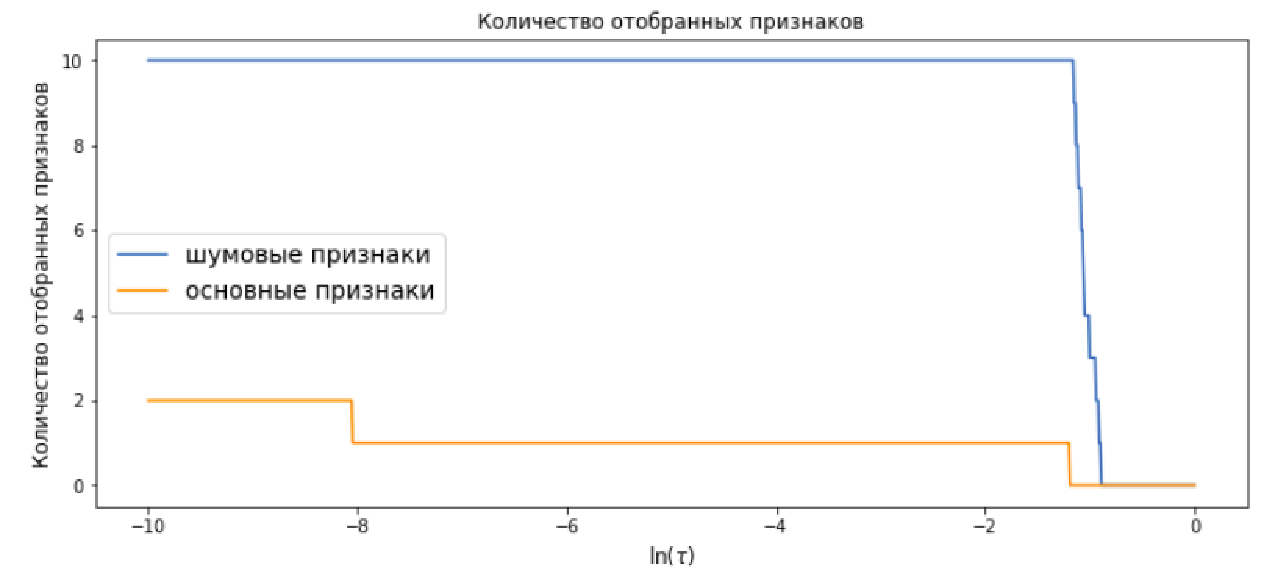
\includegraphics[width=17cm]{first_exp.pdf}}
\caption{результаты первого эксперимента}
\label{first_exp}
\end{figure}

\subsection{Стабильность модели}
Стабильностью модели будем называть отношение $\lambda_{\max}(\bX\getT\bX) / \lambda_{\min}(\bX\getT\bX)$, где $\lambda_{\min}$ и $\lambda_{\max}$ ~--- минимальное и максимальное собственные чиcла соответствующей матрицы.

В статьях \cite{Katrutsa15, KatrutsaS17},  стабильность модели имеет самостоятельную ценность и наряду с качеством прогноза на тестовой выборке определяет решение о превосходстве одного метода отбора признаков над другим. В данной работе предлагается рассматривать стабильность как априорное знание, которое указывает на то, что априори мы считаем, что выборки с меньшим числом обусловленности на множестве активных признаков появляются чаще в рассматриваемой задаче, чем выборки с большим числом обусловленности. При отсутствии такого знания стабильность стоит рассматривать в контексте повышения качества прогноза: если низкая стабильность модели ведет к снижению качества прогноза, стоит добавить штраф за низкую стабильность модели. А если качество не снижается, а повышается при уменьшении стабильности, то не стоит отдавать предпочтение менее качественной, но более стабильной модели. 

Обозначим через $\bX(\bw)$ сужение матрицы признаков на множество признаков $j:\:w_j \neq 0$. Примером соответствующей задачи оптимизации, где есть априорное знание о том, что низкое число обусловленности более предпочтительно, является задача 
$$
\|\by - \bX \bw\|_2^2 + \tau \lambda_{\max}(\bX(\bw)\getT\bX(\bw)) / \lambda_{\min}(\bX(\bw)\getT\bX(\bw)) \to \min_{\bw},
$$
что соответствует показательному распределению на числе обусловленности активных признаков выборки с гиперпараметром $\tau$. В таком виде задача является слишком трудной для оптимизации и требует перебора наборов активных признаков, например, с помощью генетического алгоритма.

\subsection{Второй эксперимент}

Рассмотрим выборку $(\bX, \:\by)$ в признаковом пространстве размерности $n$. Пусть, $y \sim \cN(0, 1)$, $ \varepsilon_j \sim \cN(0, 1)$ ~-- независимые стандартно нормально распределенные случайные величины (здесь $j \in \{1, 2, ... n\}$). Положим, $x_j = y + \nu \varepsilon_j$, где $x_j$ - $j$-ый признак, а $\nu$ - некоторое заранее выбранное значение.

Оптимальная модель использует все признаки и усредняет их для получения наилучшего прогноза целевой переменной: $\bw^* = (1 / n,\:\ldots,\:1 / n)\getT$.

Исследуем зависимость числа обусловленности $\eta$ от параметра $\nu$. При каждом значении параметра $\nu$ будем находить число обусловленности соответствующей матрицы и усреднять результат по 100 итерациям генерации целевого вектора и выборки. На каждой итерации размер целевого вектора и выборок по каждому из признаков полагаем равным 100.

\begin{figure}[htb]
\center{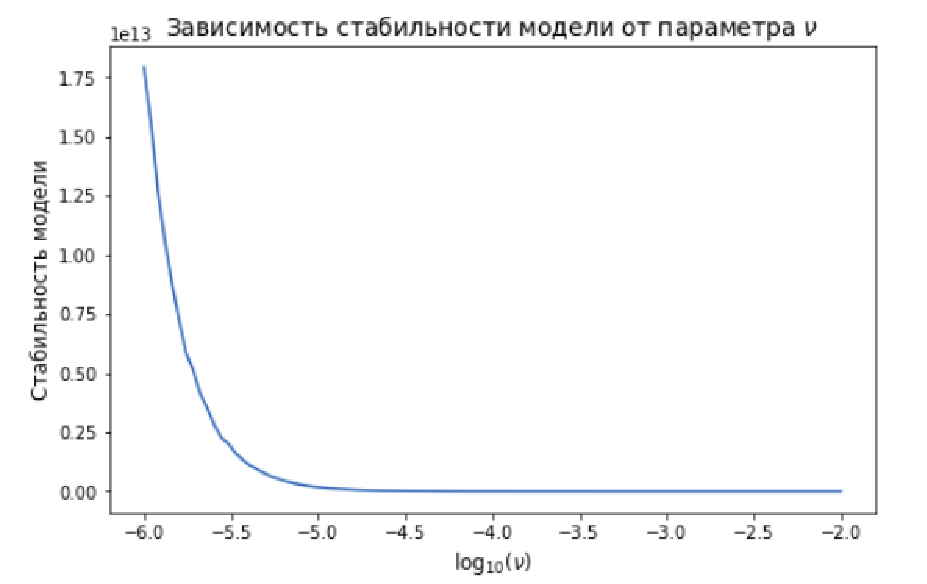
\includegraphics[width=17cm]{stab_exp.pdf}}
\caption{Зависимость стабильности модели от параметра $\nu$}
\label{first_exp}
\end{figure}

Получаем, что число обусловленности $\eta = \lambda_{\max}(\bX(\bw)\getT\bX(\bw)) / \lambda_{\min}(\bX(\bw)\getT\bX(\bw))$ при малом $\nu$ может быть большим.


\subsection{Третий эксперимент}

Пусть в выборке есть дублирование признаков. Снова положим, что целевой вектор имеет стандартное нормальное распределени: $y \sim \cN(0, 1)$. Признаки $x_1$ и $x_2$ получим как $x_1 x_2 = y + \nu \varepsilon$, где $\varepsilon \sim \cN(0, 1)$.

В этом случае число обусловленности равно $\infty$ и имеется неоднозначность решения, минимизирующего $\|\by - \bX \bw\|_2^2$. Однако все эти решения имеют $w_1 + w_2 = C = \mathrm{const}$, а потому если на тестовой выборке признаки 1 и 2 останутся идентичными, качество прогноза будет одинаковым независимо от того, какое разбиение этой константы между $w_1$, $w_2$, мы предпочтем. Обычно для того, чтобы сделать решение однозначным, добавляют слабую квадратичную регуляризацию на $\bw$ для того, чтобы из всех решений более предпочтительным было то решение, где $w_1^2 + w_2^2$ минимально, то есть $w_1 = w_2 = C / 2$. 

Заметим, что если есть основания полагать, что сильная мультиколлинеарность в обучающей выборке не будет продолжена в тестовой (см. ~\cite{multicollinearity_need_no_continuation}), то специальная обработка муьтиколлинеарности приобретает важность, а конкретный вид поправок зависит от предположений об эволюции корреляций.


\section{Заключение}
В данной работе был проведен анализ QPFS, который осуществляет отбор признаков на основе метода квадратичного программированияыла Была показана связь метода QPFS с Lasso-моделью для линейной регресии, и теоретически и экспериментально подтверждены недостатки метода QPFS на синтетических данных. Рассмотрены возможности применения числа обусловленности как априорного знания в рассматриваемой модели.

В дальнейшем планируется рассмотреть возможности применения байесовского подхода к методу QPFS для задачи отбора признаков.


\bibliographystyle{plain}
\bibliography{Tolmachev2021BayesApproach.bib}
\nocite{*}

\end{document}
